% General Presentation:
% 
%     Body text in a minimum 12 pt Times New Roman font
%     Single-spaced, with no more than 6 lines of type per inch
%     All margins set at a minimum of 3/4" (1.87 cm)
% 
% Your file must meet the following specifications:
% 
%     PDF format (.pdf extension); unprotected
%     Maximum file size of 10 mb
%     8 ½" x 11" (216 mm x 279 mm) or A4 (210 mm x 297 mm)
%     Maximum 5 pages

%     References maximum 2 pages



%\documentclass[compact]{nserc} % use xelatex
\documentclass[compact]{nserc} % use xelatex
\usepackage[]{csquotes}
\author{Guillaume Majeau-Bettez}
\addbibresource{references.bib} % cited entries only; see README for how to regenerate from Zotero


\begin{document}
\noindent \textbf{Description of the Research Program}

\begin{markdown}
%

%% What worked 7 years ago
%
% Intro: 2 pages
% Objective: 1 page with figure
% Methods (tasks and Phds): 1.75 pages
% significance and impact: 0.25 
%
% Criteria:
	% Scientific excellence of researcher
	% merit of proposal
		% originalit
		% significance
		% clarity
		% feasibility
		% consideration of EDI where relevant
		%\& 

Context, motivation, and aim
=============================

National energy and decarbonization policies, along with international climate agreements, are largely guided by large-scale energy and climate modelling tools such as Energy System Models (ESMs) and Integrated Assessment Models (IAMs).\ci{Pauliuk2017} The global IAM modelling community has converged on a manageable number of representative socioeconomic and climate mitigation pathways (Shared Socioeconomic Pathways (SSPs) and Representative Concentration Pathways (RCPs)) mapping different types of internally consistent potential futures.\ci{oneillNewScenarioFramework2014} Similarly, governments and industrial groups define roadmaps toward circular economy targets based on macro-scale material flow analyses (MFAs).\ci{aistRoadmapIronSteel2025,alonsoWorldMineralsOutlook,canadaplasticspactRoadmap2025Shared2021} These tools are designed to guide economy-wide decisions, such as national investment, taxation, and waste management policies. However, they lack the resolution to inform the everyday trade-offs made by industries and consumers. In other words, these macro-models have allowed for the development of useful global transition scenarios, but they are too coarse to offer specific guidance to the thousands of individual decisions that contribute to their implementation.

Such micro-scale environmental sustainability decisions are instead increasingly guided by a family of Attributional Life-Cycle Assessment (ALCA) tools, which estimate the share of environmental impacts that can be linked directly or indirectly to a specific product or function.\ci{Hellweg2014,hellwegLifecycleAssessmentGuide2023} Carbon footprints, environmental product declarations, and organizational LCAs are now broadly employed in product design, corporate reporting, and sustainable consumption guidance. In their common application, these assessments are mostly _retrospective_ analyses, relying on past observation data. In a rapidly transitioning economy, this reliance on near-present descriptions of processes and value chains limits the ability of decision makers to use ALCA results for forward-looking strategic decisions.

Recently, prospective-ALCA (p-ALCA) databases such as PREMISE have begun incorporating macro-model scenario data into their process, market mix, and value chain descriptions.\ci{sacchiPRospectiveEnvironMentalImpact2022} These developments bring greater temporal consistency for the environmental sustainability assessment of long-lived products and future investments.

Major inconsistencies persist, however, between p-ALCAs at the micro-scale and transition models at the macro-scale. Energy systems illustrate the problem clearly. If an industry operates in a region already supplied by clean electricity, its p-ALCA results will show a limited contribution of electricity consumption to its footprint, and therefore limited benefits in further improving its energy efficiency. Yet, energy system models often identify efficiency gains in these same industries as essential for freeing clean electricity capacity to decarbonize other sectors. What appears negligible in a static footprinting assessment can thus be critical in the dynamic transition context. These contradictions arise because p-ALCAs remain attributional in nature: they are temporally consistent with future-oriented studies but limited to the direct value chains under study, and thus cannot capture market-mediated or system-wide consequences that shape the overall transition.\ci{Heijungs2001,Majeau-Bettez2017attribCons}

Material cycles reveal a similar issue. A p-ALCA might, for instance, recommend maximizing the recycled content of a product, while dynamic material-flow analyses (dyn-MFAs) reveal that limited in-use stocks will constrain recycling supply for years.\ci{Pauliuk2015TakingStock} Increasing recycled content in one product may simply divert scarce secondary material from another, yielding little overall benefit.% These inconsistencies arise because all ALCAs are fundamentally unconstrained, linear models;\ci{Heijungs2001} they do not capture material or resource limits that are central to macro-scale transition strategies.

This is a major concern. Environmentally proactive industries that use LCAs want their performance indicators to ensure they are aligned with ---and can thrive within--- the broader sustainability transition. In other words, decision-makers need assessment tools that can capture the specificity of their system (micro-scale) in anticipating (prospective) how their decisions will contribute or hamper the broader efforts (consequences) toward achieving the environmental sustainability transitions.

Capturing constraints and market-mediated mechanisms has long been the aim of so-called Consequential LCAs (CLCAs), which focus on quantifying the direct and indirect environmental _consequences_ of decisions (or changes) in production and consumption.\ci{Zamagni2012} In short, whereas attributional LCAs describe how impacts are distributed within the value chains of a current economy, consequential LCAs quantify how impacts change when the economy itself is perturbed.\ci{Ekvall2004} Prospective variants of each extend these logics into the future, combining temporal foresight with causal reasoning.

Yet, despite being theorized already in the early 2000s,\ci{Ekvall2004} CLCAs remain a niche modelling approach.\ci{bamberComparingSourcesAnalysis2020} CLCAs require practitioners to identify which industries would respond to a change in the demand level for each product (marginal providers) and which would not.\ci{Weidema2003} This, of course, is highly uncertain and context-dependent.\ci{Mathiesen2009} Without a common framework, each practitioner was left to define ad hoc scenarios (which are subjective and hard to compare), rely on very limited empirical data, or restrict their detailed modelling to a small part of the product system (the foreground), leading to inconsistencies with background databases representing the rest of the economy. So far, building CLCAs has proven time-consuming and expensive, with results that were often difficult to interpret and viewed with skepticism.

Furthermore, CLCAs are almost invariably defined relative to one system scenario: assuming that the status quo prevails over the duration the decision under study.\ci{Steubing2016} This static assumption is ill-suited for major investment and production decisions in a rapidly evolving economy. A more robust approach, which this project proposes to develop, is to define CLCAs as perturbations around a series of representative base scenarios, each describing an internally consistent and plausible vision of the future. This ensures that consequential analyses remain coherent with broader transition pathways without relying on a single assumed trajectory.



Overarching objective and strategy
==================================

The current project is based on the hypothesis that these limitations can be overcome by embedding CLCA development in a shared framework of prospective scenarios, tightly linked to the frameworks already developed for macro-models (SSPs, RCPs, etc.), and transparently leveraging a wide range of modern Big Data sources. In other words, we aim to develop a reproducible framework and an ambitious data fusion approach for efficient, robust, and data-rich prospective CLCAs (p-CLCA). This will constitute a radical shift and a new perspective in LCA practice: rather than simply describing a product’s performance in a given future (as in p-ALCA) or estimating marginal shifts around today’s system (as in CLCA), our approach evaluates specific decisions in terms of their ability to facilitate or counter a manageable set of representative transition pathways. This enables consistent articulation between micro-scale decisions and macro-scale scenarios for achieving environmental sustainability goals.


Research frontier and strategy
==============================



\underline{A pragmatic but consistent approach:~} Multiple individual prospective case studies present some consequential aspects in the modelling of their system of interest (the \enquote{foreground}). However, as reviewed by Nurdiawati et al, \cite{nurdiawatiRecentAdvancementsProspective2025}, these studies have to rely on LCA databases that describe the rest of the economy (the \enquote{background}) based on assumptions that contradict the consequential and prospective nature of the overall study, leading to inconsistencies. In the context of LCA, the foreground refers to the specific system or product being studied, while the background encompasses all other interconnected processes in the broader economy represented in databases such as ecoinvent. This project will jointly tackle background database (Tasks~1 and~2) and foreground (Task~3) modelling in a single, consistent framework. A pragmatic, iterative approach will initially leverage global scenarios and datasets in defining prospective, consequential background databases; while performing more detailed data mining and prospective modelling of market dynamics and constraints for the foreground consequential system.

\underline{Reconciliation and disaggregation of core scenario variables:~} Recent exploratory work by Maes et al.\ci{maesProspectiveConsequentialLife2023} presented different ways of defining a marginal/consequential electricity mix starting from projected IAM production mixes. These techniques, however, do not fully leverage all the available scenario data. Our approach will combine multiple layers of information ---installed capacities, projected additions, efficiency improvements, and regional availability--- to identify how each technology or region responds to changing demand. We will notably rely on the installation of novel capacity to define long-term marginal technologies, and on unused capacity to identify short-term consequences to a change in demand. By reconciling scenario data with each region’s characteristics and currently installed capacities, we will obtain regionalized and technologically disaggregated transition pathways, matching the resolution of LCA databases.

\underline{Coverage rather than specificity in the background:~} The detailed development of baseline scenarios for the future of \emph{each} material or energy carrier could constitute its own PhD project. Yet, to be useful in p-CLCA database development, these scenarios must be applied to a broad coverage of energy types and materials. Pragmatic simplifications and modelling choices will therefore need to be made in Tasks~1 and~2 to initially prioritize coverage, followed by iterative refinements of scenario definitions and models. This staged approach ensures early functionality and breadth, while leaving room for depth as methods and data mature.

\underline{Inclusivity and diversity in scenario development} The development of representative scenarios for the future is at the heart of prospective analyses. This is a highly subjective endeavour, with a high risk of blindspots in scenario coverage. For example, the major IAMs have been criticized for not including a degrowth-based scenario among the core SSPs,\ci{debortoliMoreRationalityInclusivity2025} which all exogenously assume a pursuit of economic growth. In this project, we plan to largely build upon existing scenario development work. That being said, the core defining characteristics of the different representative scenarios will have to be extended, notably to link these mostly-energy-focused narratives with material roadmaps. Ensuring diverse perspectives in this step reduces the risk of systematically biased or incomplete assumptions.\ci{debortoliMoreRationalityInclusivity2025} What level of dematerialization, of international trade and collaboration surrounding critical materials, or of dismantling and recycling effort can we envision for the future? In identifying these defining characteristics of the prospective scenarios that serve as starting point for our consequential LCA modelling, we will strive to build a broad consensus from the perspectives of a diverse panel, reflecting stakeholders from different origins (all continents), career roles (in academia, in industry, as citizen/consumers, etc.), genders and age.

\underline{Open digital infrastructure:~} The proposed framework will be developed from day~1 in an open-source manner. It will cover every step from data extraction to final analysis in a modular and transparent manner. By avoiding manual steps and relying on reusable algorithms and code, it will facilitate its maintenance over time, its broader adoption by the community  and its iterative improvement. The resulting open-source toolkit for data fusion, scenario definition, and p-CLCA generation will not only support this project but also enable reproducible, collaborative research across institutions and countries. In fact, the digital infrastructure will constitute a core deliverable of the project, following the growing trend toward open-source software-based sustainability science.


Methods and proposed approach
=============================

\begin{figure}[h]
	\centering
	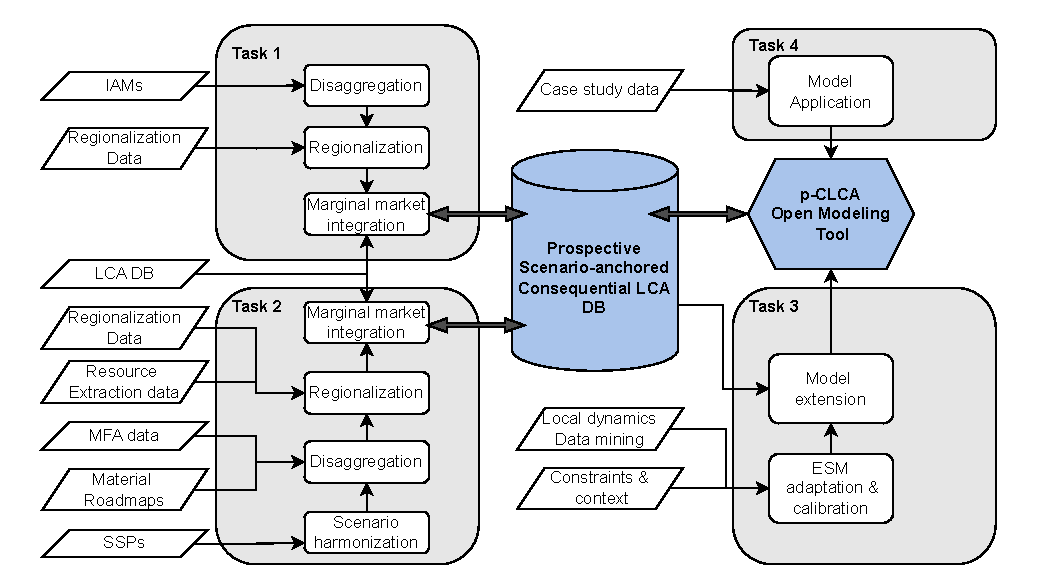
\includegraphics[width=0.8\textwidth]{discovery.drawio.pdf}
\end{figure}

## Task 1 -- Transform LCA background databases for prospective-consequential studies following energy transition scenarios (PhD1)

This first task (PhD 1) will leverage a representative set of precalculated Integrated Assessment Model (IAM) energy and decarbonization scenarios to define consistent, scenario-driven consequential LCA background datasets for energy supply. Relevant scenario variables ---unused capacity, new installations, storage additions, and efficiency improvements, etc.--- will be extracted and regionalized to match the resolution of major LCA databases such as ecoinvent. Short-term consequences will be derived from unused or idle capacity, while long-term consequences will reflect new capacity additions and retirements. This two-tiered treatment captures both rapid and structural responses of the energy system to changes in demand. By reconciling scenario data with regional characteristics (e.g., resource availability, grid composition, and technology mix), the project will generate regionalized, temporally explicit, and scenario-consistent marginal mixes for electricity, heat, fuels, and biofuels. These will form the energy backbone of the prospective-consequential framework and directly feed subsequent modelling tasks. This work builds upon our ongoing methodological exploration of how IAM data can inform consequential modelling.\ci{provost-savardGuidelinesProspectiveConsequential2025}



## Task 2 -- Transform LCA background databases for prospective-consequential studies following material circularity transition scenarios (PhD2)

The second task (PhD 2) mirrors Task 1 but focuses on materials rather than energy. It will cover critical and major metal groups, polymers, food, and construction materials, using available global roadmaps and extraction projections. Because material extraction and processing are closely intertwined with energy transitions, aligning material scenarios with IAM-based energy pathways is essential for overall consistency. A first sub-objective will therefore be to reconcile diverse material forecasts and circular-economy roadmaps with the energy-system scenarios employed in Task 1. Our group has already demonstrated such an alignment for aluminium scenarios,\ci{pedneaultSectorspecificScenariosFuture2022} which can be generalized and extended to other materials.

Following this alignment, the project will disaggregate material scenarios by region and sub-technology, estimating how changes in material demand perturb these trajectories. This will yield marginal technology and market mixes for the prospective-consequential LCA database. The modelling will integrate the dynamics of material stocks and recycling flows, building on open-source material-flow-analysis software and datasets.\ci{Pauliuk2015TakingStock} Given the diversity of materials and the more fragmented nature of circular-economy projections compared to energy scenarios, the initial level of detail may be lower than in Task 1, but pragmatic data-fusion strategies will ensure broad coverage. The resulting datasets will extend the p-CLCA database to material systems, identifying time-dependent marginal suppliers under resource constraints across representative scenarios.



## Task 3 -- Develop p-CLCA modelling tool for data-rich foreground analysis of specific decisions scenarios (PhD3)

As Tasks 1 and 2 focus on the development of generic p-CLCA processes, it makes sense that these rely on the pre-calculated results from macro-scale models. For many decision contexts, the background p-CLCA databases developed in Tasks 1 and 2 will already provide micro-scale results that are both internally consistent and aligned with transition objectives. However, some systems exhibit complex feedbacks, resource constraints, or multi-sector interactions that cannot be represented by linearly combining marginal impacts from the background database. Task 3 (PhD 3) therefore extends the framework to explicitly represent these dynamic and interconnected systems, structuring how p-CLCA can handle non-linear responses and system feedbacks in a transparent and reproducible way.

To capture these interactions, the framework will simulate the evolution of a representative regional system over time ---with and without a given decision--- using an energy-system model calibrated for a Canadian province (e.g., Québec). The differences between these two simulations thus provides an estimate of the net consequences of the decision. This model will be extended to include material requirements, trade, land-use constraints, and environmental emissions, thereby capturing how a single decision in one sector can propagate across others. Repercussions that extend beyond the regional boundaries will be estimated from the global p-CLCA databases developed in Tasks 1 and 2, ensuring consistency between regional and global transition pathways.

We aim for a foreground modelling framework that can be applicable to different regions, and that can capture a broad range of technological, production, and consumption choices. This first implementation will build on the EnergyScope-Québec model, an existing energy-system model already coupled with LCA and progressively integrating material flows and constraints. The PhD student will strengthen this representation through extensive data-mining on industrial processes, material supply chains, and regional trade statistics. A major deliverable will be a standardized protocol connecting dynamic regional models to global p-CLCA databases—reconciling historical trade data with scenario-based projections of imports and exports. This ensures that Task 3 develops not only a regional application but also a transferable methodological layer for dynamic decision analysis within the broader p-CLCA framework.


## Task 4 -- Demonstration and deployment (MSc 1 and 2)

Two MSc students will be responsible for the first demonstration and deployment of the developed p-CLCA framework. These activities will serve as proof-of-concept studies, validating the methodological and data-integration components established in Tasks 1–3 while also generating practical insights for real decision contexts. One project will focus on the transformation of an industrial process (e.g., electrification, decarbonization of heat supply, or substitution of feedstocks), and the other on the eco-design of a consumer product (e.g., low-carbon construction material). Both will apply the full prospective-consequential workflow—from scenario selection to data fusion and impact interpretation—to assess how concrete technological or design choices influence transition trajectories.

Beyond validation, Task 4 also plays a synthesis role. The MSc researchers will document methodological and data gaps encountered during application, feeding these insights back into framework refinement. They will collaborate closely with industrial and institutional partners within the CIRAIG network, ensuring the framework’s usability for real-world decision support. The combined outcomes of these demonstration projects will illustrate how the proposed methodology enables more robust, forward-looking sustainability assessments and provide open, reproducible case studies to foster future adoption and teaching.



Links to recent progress in the applicant's research activities
===============================================================

This ambitious program launches from a strong foundation of recent advances within our group, positioning us to tackle the next methodological frontier in LCA. Task~1 will extend the methodological guidelines we recently developed for integrating IAM scenario data into prospective consequential LCA modelling,\ci{provost-savardGuidelinesProspectiveConsequential2025a} transforming them from conceptual principles into a robust computational framework for energy transition pathways. Task~2 builds on our modelling of metal flows, stocks, and resource constraints associated with future energy trajectories (accepted at _Nature Sustainability_),\ci{bieuvilleMetalBottlenecksEnergy2025} as well as our open digital infrastructure for regionalizing and spatializing LCA databases\ci{agezCIRAIGRegioinventRegioinvent2025} --- now repurposed to support global-scale data fusion. Task~3 will expand the coupling of energy and material systems we initiated while calibrating the EnergyScope–Québec model,\ci{limpensEnergyScopePathwayOpensource2024, limpensEnergyScopeTDNovel2019a} advancing it toward a dynamic, data-rich decision-analysis framework capable of representing feedbacks across sectors.\ci{souttreMescalToolCoupling2025} Finally, Task~4 will draw on our established collaborations with industrial partners through the CIRAIG International Research Consortium on Life Cycle Assessment and Sustainable Transition, ensuring that the new framework is tested and refined in realistic, high-impact contexts.


Importance and impact of research
====================================

This project arrives at a watershed moment for the life cycle assessment (LCA) community. As national and international efforts toward decarbonization accelerate, the limitations of current LCA methods have become increasingly apparent: attributional and even prospective tools provide detailed but often disconnected pictures of sustainability performance. The proposed framework for prospective consequential LCA (p-CLCA) represents a fundamental shift—moving beyond static or retrospective assessments to models that explicitly quantify how individual decisions alter the broader physical economy and its transition pathways. By linking LCA practice with scenario-based macro-modeling traditions (e.g., IAMs, ESMs, and MFAs), this research will help redefine how environmental scientists and engineers conceptualize system boundaries, causality, and temporal dynamics in sustainability assessment. The open and reproducible digital infrastructure developed here will also serve as a shared foundation for future work, fostering transparency, interoperability, and collective progress across the international LCA community.

For industrial and societal decision-makers, the proposed framework provides a much-needed bridge between high-level transition scenarios and practical, operational guidance. It will allow companies and governments to test whether their strategies are genuinely aligned with realistic decarbonization and circular-economy trajectories, rather than assuming endless supplies of clean energy or recycled materials. The resulting tools and databases will enable more robust risk assessments and long-term investment planning, improving the credibility of sustainability claims and reducing the likelihood of lock-ins or rebound effects.

Strategically, this project will contribute directly to Canada’s commitment to achieve net-zero greenhouse gas emissions by 2050, as outlined in the 2030 Emissions Reduction Plan and Canadian Net-Zero Emissions Accountability Act. Canada’s resource-rich economy, regionally diverse energy systems, and export-oriented industrial base create both opportunities and constraints for deep decarbonization and circularity. Achieving these goals will require decisions that are not only efficient within sectors, but also coherent across regions, supply chains, and time horizons--a challenge that this project directly addresses. By providing open, data-driven methods to connect Canadian industrial realities with global transition pathways, this research will strengthen the analytical foundations of national initiatives such as the Canadian Critical Minerals Strategy, Clean Growth Strategy, and 2030 Agenda for Sustainable Development.

Finally, by developing transparent, open-source tools and training a new generation of highly qualified personnel in advanced sustainability modelling, this program will help Canada build enduring capacity for evidence-based environmental decision-making. In doing so, it positions Canadian researchers and industries not only to adopt but to help shape the next generation of sustainability assessment tools—ensuring that Canada’s transition to a low-carbon, resource-efficient economy is scientifically grounded, globally connected, and resilient.

\end{markdown}

\pagebreak
\setcounter{page}{1}
% Renew geography
\newgeometry{left=1.9cm, right=1.9cm, top=1.9cm, bottom=1.9cm, headheight=15pt}
\begingroup
\setlength\bibitemsep{0pt}
%\begin{multicols}{2}
\printbibliography
%\end{multicols}
\endgroup

\end{document}

% focus on therefore generate a consequential LCA database to represent the evolution of marginal providers based on each SSP/RCP pathway model. With this approach, an industry assessing a possible choice will be able to evaluate to what extent the environmental consequences of its decision are sensitive to the evolution of the rest of the economy. This task will require a major spatial and technological disaggregation of IAM results, notably for the energy, transportation, and agricultural sectors.

%\begin{wrapfigure}[20]{r}{0.5\textwidth}
%\centering
%\includegraphics[width=0.5\textwidth,draft=false]{fig_researchPlan.pdf}
%\label{figPlan}
%\end{wrapfigure}

%% TODO: scope limitations? process scale-up 

%Together, these achievements provide a proven platform from which this project can push methodological boundaries. Rather than consolidating existing approaches, the proposed work uses them as launchpads for a step-change in how environmental consequences are modelled --moving from static inventories toward dynamic, scenario-consistent representations of sustainability transitions.
